\documentclass{llncs}
\usepackage{times}
\usepackage[T1]{fontenc}

\usepackage{a4}
\usepackage[margin=3cm,nohead]{geometry}
\usepackage{epstopdf}
\usepackage{graphicx}
\usepackage{fancyvrb}
\usepackage{amsmath}
\usepackage{wrapfig}
\renewcommand{\baselinestretch}{1.5}

\usepackage[utf8]{inputenc}
\usepackage[portuges]{babel}


\begin{document}
\mainmatter
\title{Mobile Networks: From 4G to 5G}

\titlerunning{Mobile Networks: From 4G to 5G}

\author{João Teixeira \and José Ferreira \and Miguel Solino}

\authorrunning{João Teixeira \and José Ferreira \and Miguel Solino}

\institute{
Universidade do Minho, Departamento de  Informática, 4710-057 
Braga, Portugal\\
e-mail: \{a85504,a83683,a86435\}@alunos.uminho.pt
}

\date{}
\bibliographystyle{splncs}

\maketitle
\begin{abstract}
Todos os entusiastas das novas tecnologias sonham puder descarregar
ficheiros da Internet a velocidades alucinantes.
Inevitavelmente, esse sonho acabou por sair das nossas casas e
seguir-nos para a rua à medida que os dispositivos se tornavam mais
compactos, mais potentes e mais generalizados, com cerca de 5 mil
milhões de utilizadores em 2010 \cite{Upkar12}.
A solução prontamente apresentada pelas empresas foi uma conexão
móvel cada vez mais rápida.
Eventualmente foi atingida uma barreira na procura incessante da
velocidade, o 4G. A resposta das empresas a este entrave foi o
desenvolvimento de um novo paradigma denominado de 5G.
\end{abstract}

\section{Introdução}

Este artigo irá explorar a evolução dos serviços móveis baseados em 4G
LTE para serviços móveis baseados na nova tecnologia de ponta
denominada de 5G assim como as suas vantagens e desvantagens.\\
Este \textit{paper} está estruturado da seguinte forma. Primeiro é 
feita uma breve análise dos principais pontos de evolução até à 
chegada ao 4G. Depois, a implementação do 4G e as suas consequentes 
limitações são exploradas levando à apresentação da implementação do 5G
e os problemas que este resolve.
Claro que esta tecnologia tem algumas desvantagens que também serão 
exploradas.
Por fim, serão apresentados vários projetos envolvendo 5G.

\section{Caminho para o 4G}
A fim de melhor entender as vantagens proporcionadas pelo 5G temos
de previamente conhecer a forma como a comunicação móvel tem vindo a
evoluir ao longo do tempo e compreender a norma que esta vem
substituir.\\
A primeira geração, desenvolvida durante a década de 80, era meramente
analógica permitindo velocidades de comunicação extremamente lentas.
Apesar de ser relativamente rudimentar, como o desenvolvimento deste
método foram resolvidos múltiplos problemas, tais como o multiplexing
da banda de frequências. Desde aí várias tecnologias novas foram
implementadas.\\
Com a introdução da segunda geração, na década de 1990, a comunicação
passou a ser digital e foi acrescentado o suporte para mais
utilizadores.\\
Por fim, a terceira geração introduziu maiores
velocidades de transferência\cite{Kaleem12} .\\
Por fim, com a quarta geração de comunicação móvel, denominada de 4G
LTE, existiram inúmeros avanços.
Passou a ser possível passar de uma torre para outra sem quebras de
conexão e a capacidade do sistema mais do que triplicou \cite{Choi06}.

\begin{wrapfigure}{r}{0.39\textwidth}
  \centering
  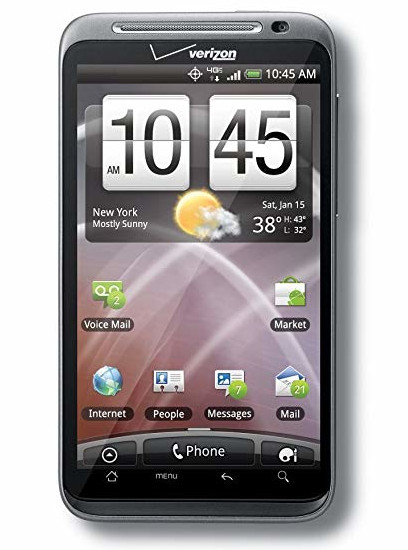
\includegraphics[width=0.30\textwidth]{images/thunderbolt.jpg}
  \caption{HTC ThunderBolt (ADR6400L)}
  \label{fig:thunderbolt}
\end{wrapfigure}

\section{Implementação do 4G}
A primeira rede de 4G LTE (\textit{Long Term Evolutin})foi implementada
em Oslo, Noruega e Estocolmo, Suécia em 2009. 
Estranhamente, apesar de existirem redes experimentais de 4G desde
2009, o primeiro telemóvel comercialmente disponível a usufruir desta
norma foi o HTC ThunderBolt (ADR6400L) \ref{fig:thunderbolt} que 
apenas saiu em 2011.\\
O \textit{standard} LTE apresenta uma velocidade máxima 
de\textit{dowlink} de 300 Mbit/s e velocidade máxima de
\textit{uplink} de 75 Mbits/s.


\subsection{A barreira do 4G}
Apenas dispositivos multi-banda conseguem ligar-se a redes móveis por
todo o mundo. Tal deve-se ao facto de que cada país utiliza uma banda
diferente.

\section{Passagem do 4G para o 5G}
A passagem do 4G para o 5G é expectavel que leve pelo menos uma
década, embora pareça uma realidade próxima, com todos os 
equipamentos que vão sendo divulgados que já possuem a capacidade
de suportar esta norma. Aos poucos, já estão a ser preparadas
condições para se torne acessível a todos, como veremos de 
seguida.

\section{Implementação do 5G}
A implementação do 5G será muito mais orientada à experiência do
utilizador, ao contrário do que se vê na norma 4G, onde o 
desempenho da rede é baseado em cobertura, velocidade de 
transferência de dados, entre outros. No 5G vai ser prioridade a
facilidade de conexão entre dispositivos próximos e eficiência
energética.\\
Para proporcionar uma melhor experiência de utilização, vai ser
introduzido um novo conceito de personalização do serviço
conforme as necessidades do utilizador, podendo dar prioridade,
por exemplo, à latencia e fiabilidade ou velocidade da conexão.

\subsection{Problemas resolvidos}
\subsection{Desvantagens inerentes}
\subsection{Utilização}
- Comunicação D2D
- Comunicação M2M
- Internet of Things
- Comunicação Automovel Avançada
- Setor de Saúde
- Outras Aplicações
\section{Projetos 5G}
\subsection{Desenvolvimento}
Conhecendo já do que se trata o 5G e as suas vantagens e evoluções,
é possível analisar as vantagens que esta nova tecnologia trás para
o utilizador comum.\\
Caso estas vantagens fossem inexistentes, não teríamos várias empresas
a dedicar os seus recursos a implementar esta tecnologia por todo o mundo.\\
Um exemplo destas empresas é a \textit{Huawei}.
É digno de nota que esta empresa está a focar parte dos seus esforços em
países em desenvolvimento, tais como Cabo Verde, Moçambique e Brasil,
levando assim a uma melhoria das infraestruturas de comunicação e, consequente,
à melhoria das condições económicas para a população. Mais concretamente,
no Brazil está previsto um investimento de pelo menos 800 milhões de euros
na construção de uma fábrica em São Paulo.
Para além do objetivo humanitário, estas medidas surgem como resposta à tão
mediática guerra comercial entre a China e os Estados Unidos.
Ao contrário dos Estados Unidos, que se recusa a aceitar a Huawei, a Rússia
recebeu de braços abertos esta tecnologia inovadora.
No caso de Portugal, já existem múltiplas empresas a querer investir no 5G,
sendo uma delas a \textit{Dense Air Portugal} que pretende distribuir esta
novidade pelo país.
Já foram feitos estudos por esta empresa que concluem, ao fim da
realização de mais de 600 mil ensaios, que pelo menos 39 mil edifícios
estão aptos para receber antenas 5G \cite{5GPortugal}.

\subsection{Dispositivos}
Enquanto as maiores empresas investem em implementar o 5G globalmente, as com
menos capacidades de realizar essa proeza preocupam-se em investir na construção
e desenvolvimento de dispositivos que utilizem esta tecnologia. Tais empresas como
Samsung, Xiaomi, OnePlus, Nokia, etc já inicializaram o processo de criação
desses mesmos no instante em que as informações necessárias foram tornadas "públicas".
Ou seja, uma corrida entre "grandes nomes" para decidir qual delas fornece os produtos
mais rápido. Obviamente que se sabe que as primeiras a produzir vão ser as mais próximas da informação como a Huawei e a Xiaomi.
Entretanto, além dos futuros responsáveis pela maior parte da utilização
do 5G, também existem diferentes nomes em outras indústrias: Qualcomm 
na produção das peças para os smartphones, AT\&T, Nokia, T-Mobile e Verizon nas
infraestruturas e Intel e DoCoMo na área dos automóveis. 
\section{Conclusões}

Neste trabalho...

%UNCOMMENT para a bibliografia 
%% ficheirodebibliografia.bib
%\bibliography{ficheirodebibliografia}

%ou inserir directamente os vários \bibitem 
\begin{thebibliography}{1}

\bibitem{Upkar12}
Upkar Varshney:
\newblock{4G Wireless Networks} (2012)

\bibitem{Choi06}
Jinsung Choi
\newblock{4G, Solution for Convergence?} (2006)

\bibitem{Kaleem12}
M.Kaleem Iqbal, M. Bilal Iqbal, I. Rasheed, A. Sandhu:
\newblock{4G Evolution and Multiplexing Techniques with solution to
implementation challenges} (2012)

\bibitem{Boyd12}
B. Bangerter, S. Talwar, R. Arefi, K. Stewart, Intel:
\newblock{Networks and Devices for the 5G Era} (2014)

\bibitem{Lauridsen17}
M. Lauridsen, L. C. Giménez, I. Rodriguez, T. B. Sørensen, P. Mogensen:
\newblock{From LTE to 5G for Connected Mobility} (2017)

\bibitem{Agiwal16}
M. Agiwal, A. Roy, N. Saxena:
\newblock{Next Generation 5G Wireless Networks: A Comprehensive Survey} (2016)

\bibitem{5GPortugal}
Dense Air Portugal está em "diálogo com Anacom" para 5G:
\newblock{https://www.noticiasaominuto.com/economia/1329407/dense-air-portugal-esta-em-dialogo-com-anacom-para-5g}
(29 de setembro de 2019)


\end{thebibliography}

\end{document}
